\documentclass[ManualeUtente]{subfiles}

\begin{document}

\chapter{University}
After logging as university, you will see this screen:
\begin{figure}[H]
	\centering
	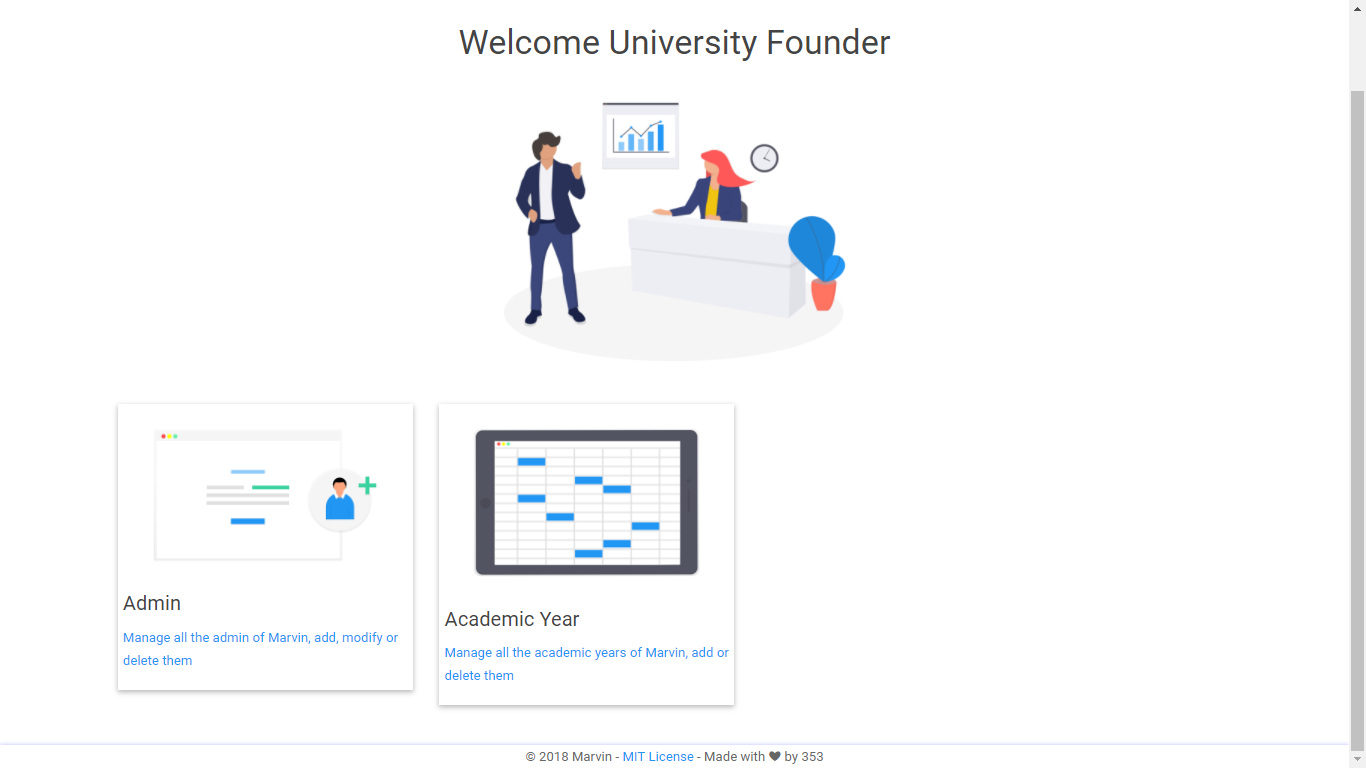
\includegraphics[width=0.7\linewidth]{./image/University}
	\caption[University]{University home page}
	\label{fig:university1}
\end{figure}
\newpage
\section{Admins management}
To manage admins, you have to click on the right section\\
\begin{figure}[H]
	\centering
	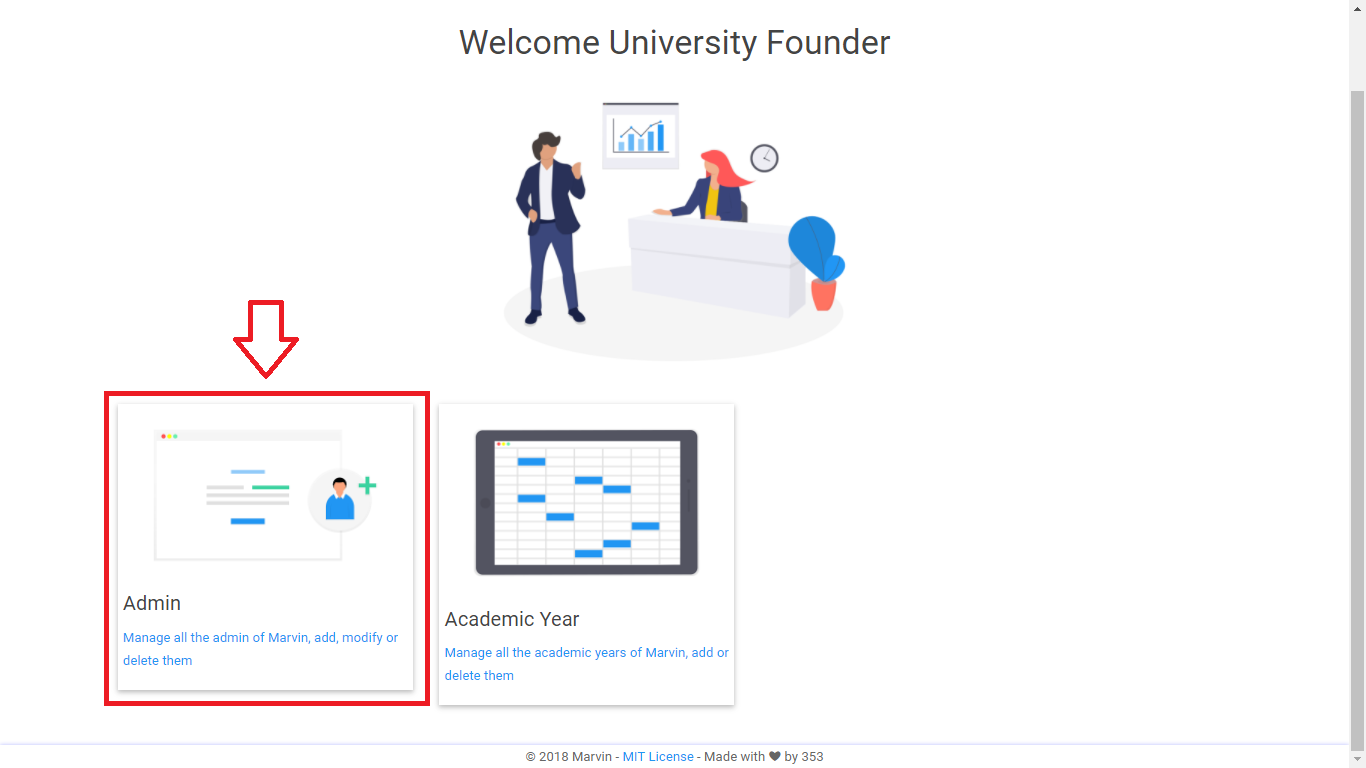
\includegraphics[width=0.7\linewidth]{./image/UniAdmin}
	\caption[Manage admin]{Manage admins}
	\label{fig:uniadmin}
\end{figure}

\subsection{Add a new admin}
\begin{figure}[H]
	\centering
	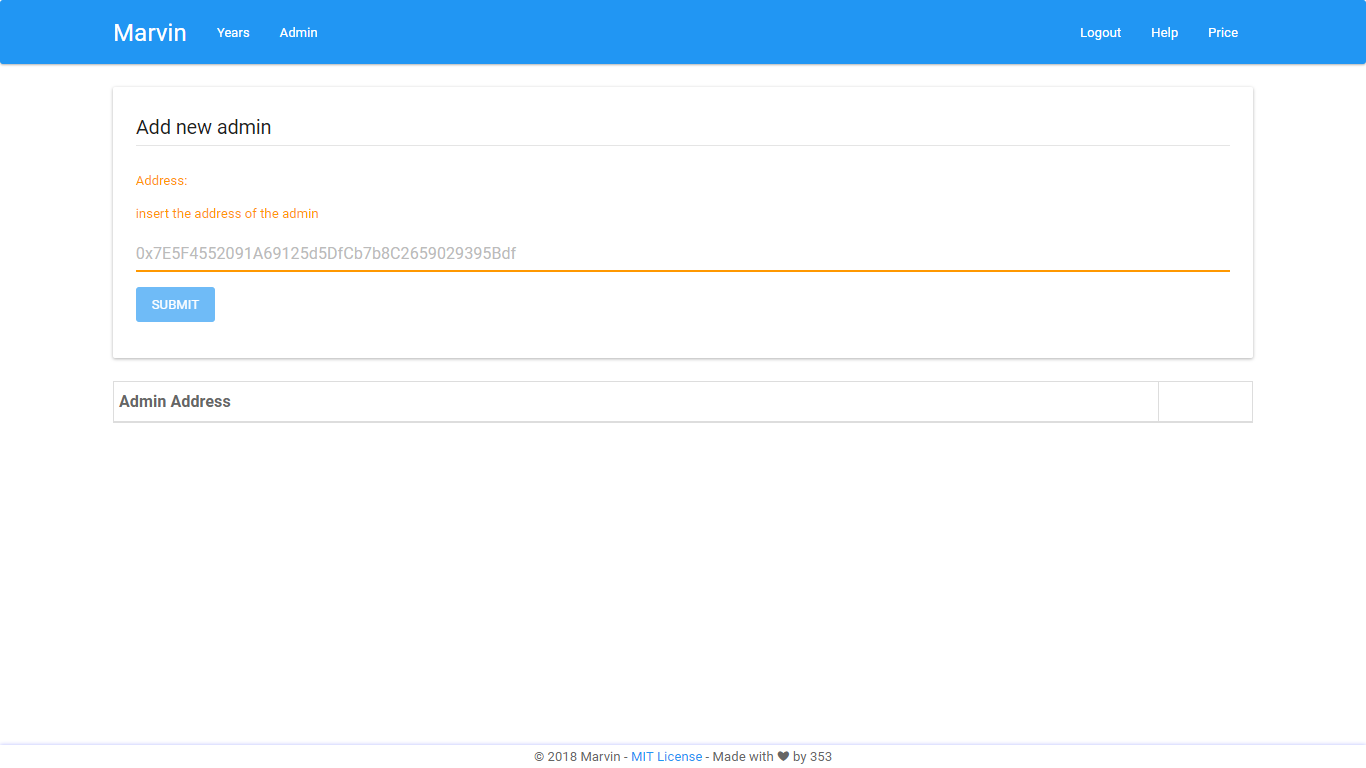
\includegraphics[width=0.7\linewidth]{image/UniversityAddAmin}
	\caption[Add admin]{Add a new admin}
	\label{fig:Add a new admin}
\end{figure}
To add a new admin, you have to go to the manage admins section and:
\begin{enumerate}
	\item Insert the admin's key in the form;
	\begin{figure}[H]
		\centering
		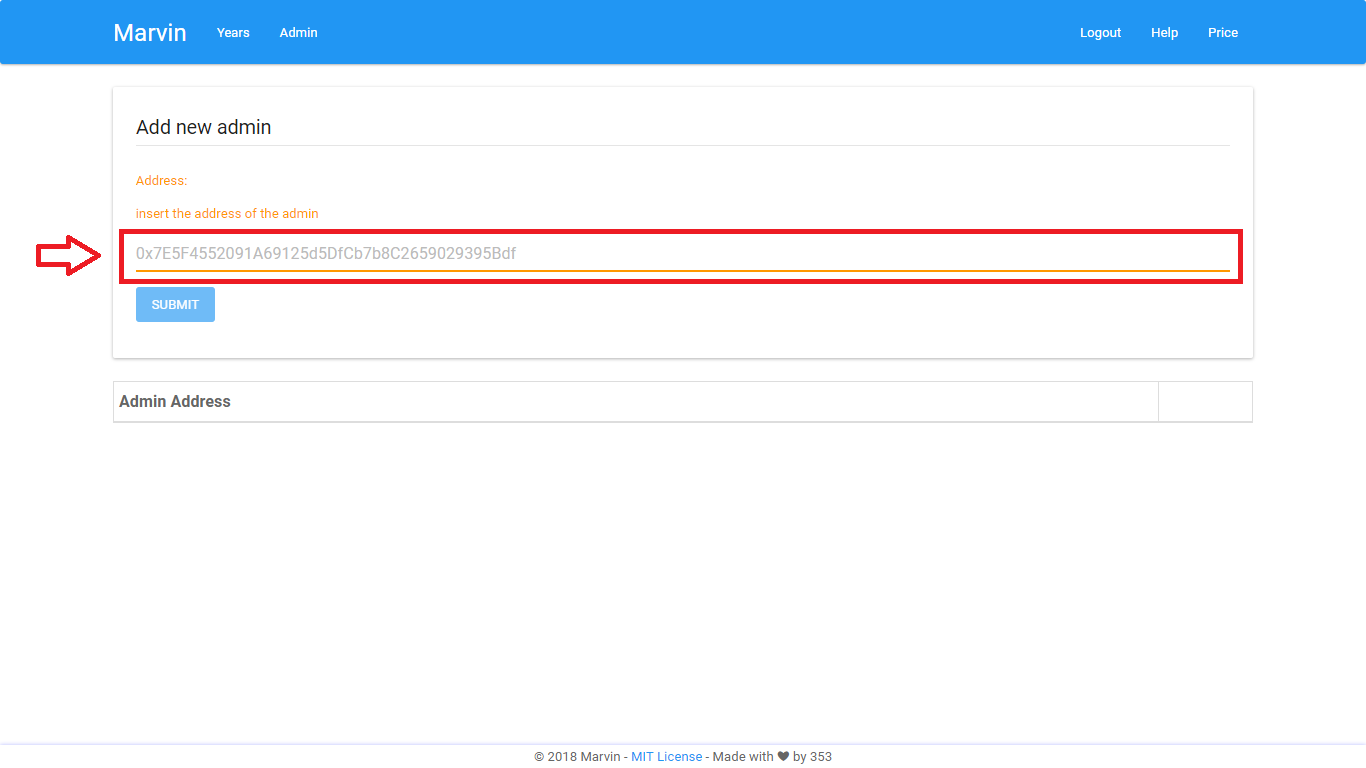
\includegraphics[width=0.7\linewidth]{image/UniversityAddAmin1}
		\caption[Add admin form]{Fill the form}
		\label{fig:Add a new admin, fill the form}
	\end{figure}
	\item Click on the button ``Submit".
	\begin{figure}[H]
		\centering
		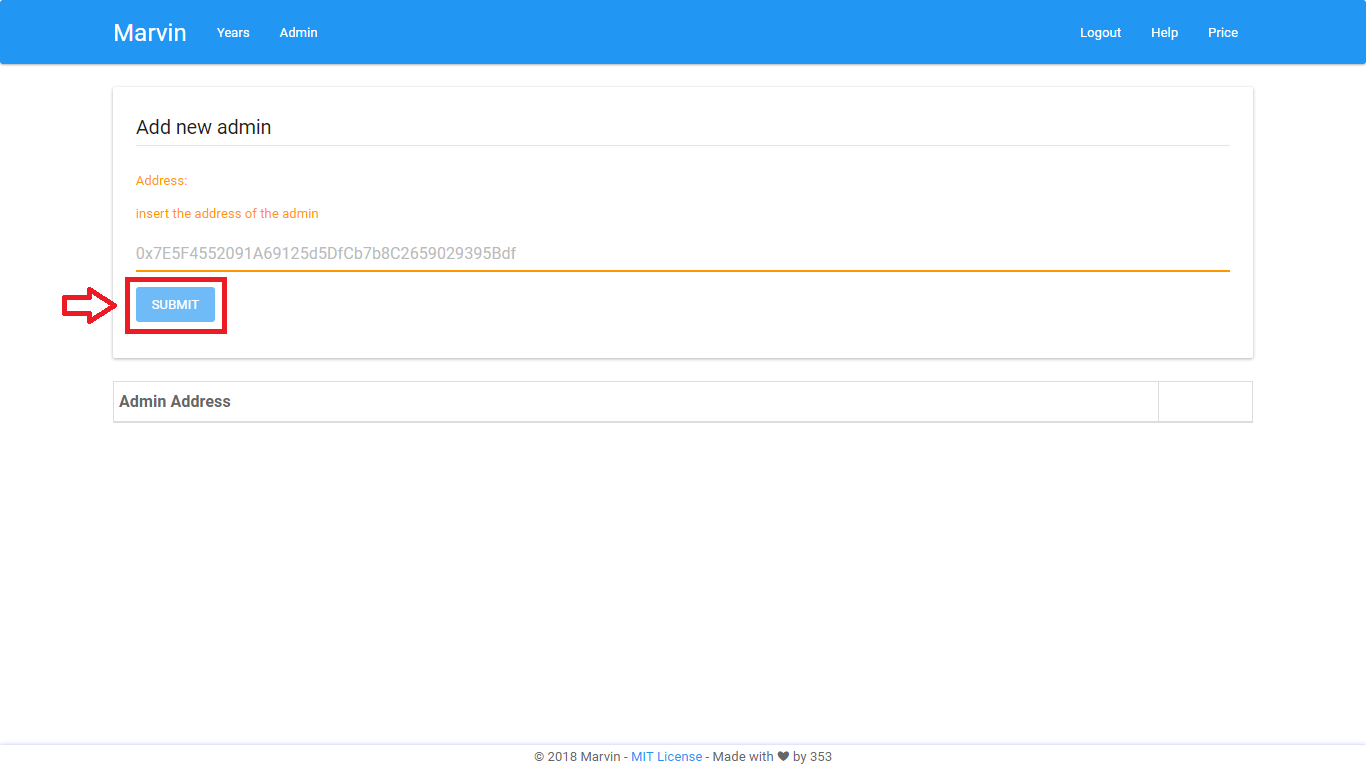
\includegraphics[width=0.7\linewidth]{image/UniversityAddAmin2}
		\caption[Add admin submit]{Click submit}
		\label{fig:Add a new admin, click submit}
	\end{figure}
\end{enumerate}

\subsection{Remove an admin}
To remove an admin, you must click on the ``Delete" button next to the admin you want to delete.
\begin{figure}[H]
	\centering
	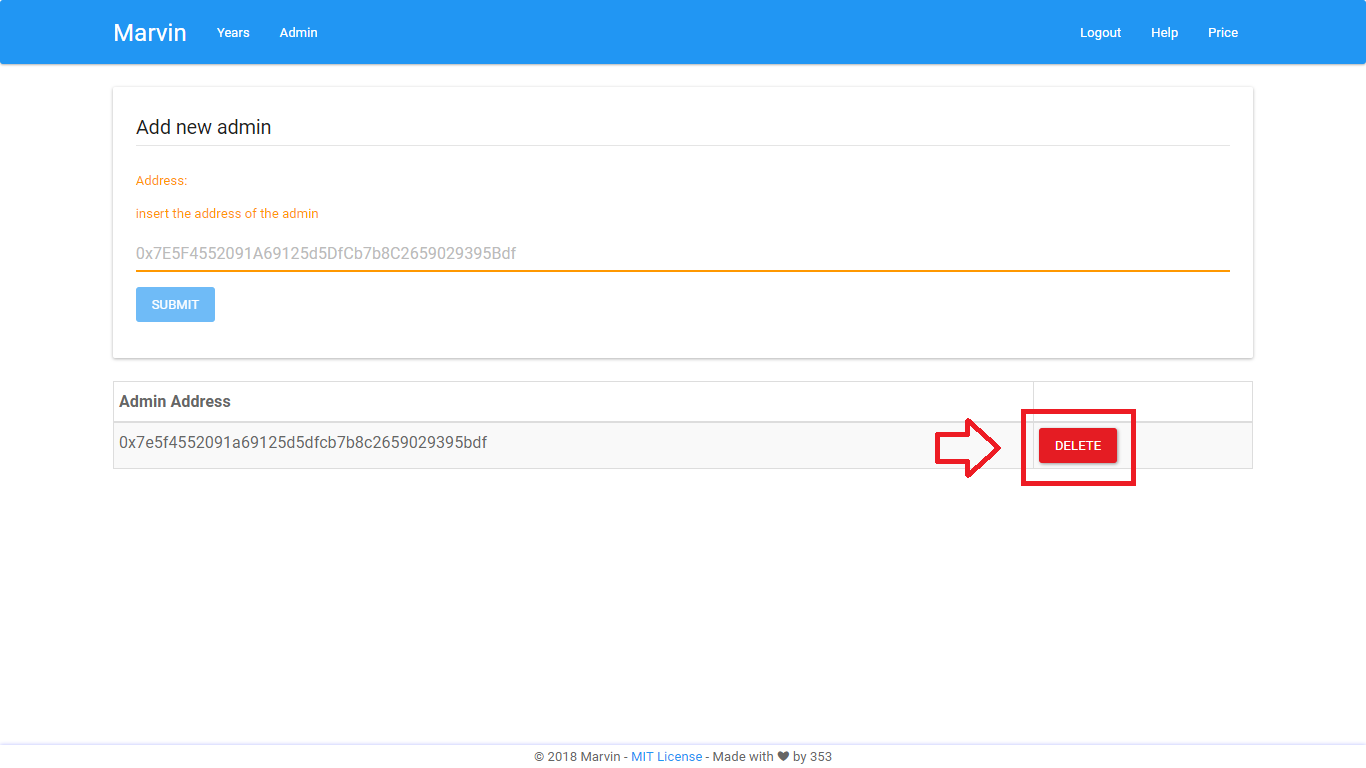
\includegraphics[width=0.7\linewidth]{image/DeleteAdmin}
	\caption[Delete admin]{Delete an admin}
	\label{fig:Delete an admin}
\end{figure}
\newpage

\section{Academic years management}
To manage academic years, you have to click on the right section.
\begin{figure}[H]
	\centering
	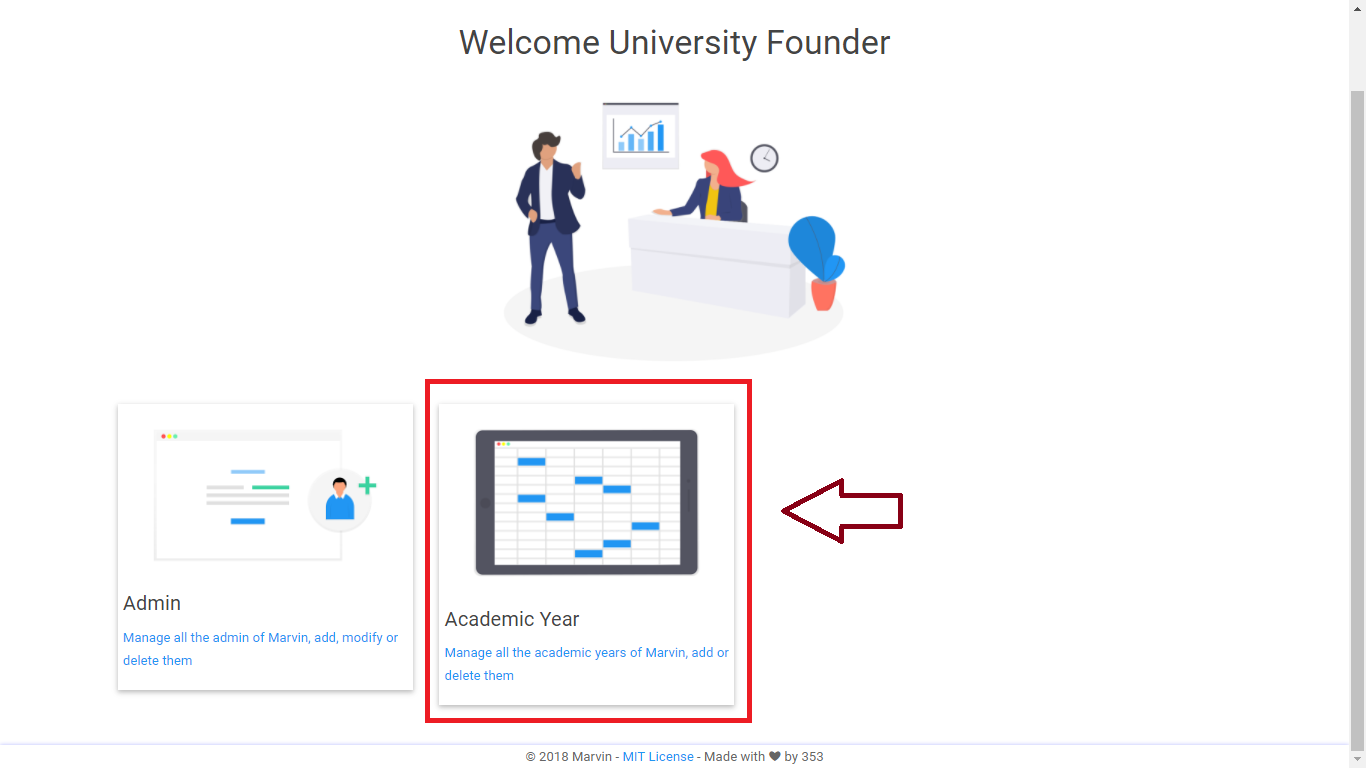
\includegraphics[width=0.7\linewidth]{image/UniAcademicYear}
	\caption[Add year]{Add a new academic year}
	\label{fig:Add a new academic year}
\end{figure}
\subsection{Add a new academic year}
To add a new academic year, you must go to the manage academic years' section and:
\begin{enumerate}
	\item Insert the new year in the form;
	\begin{figure}[H]
		\centering
		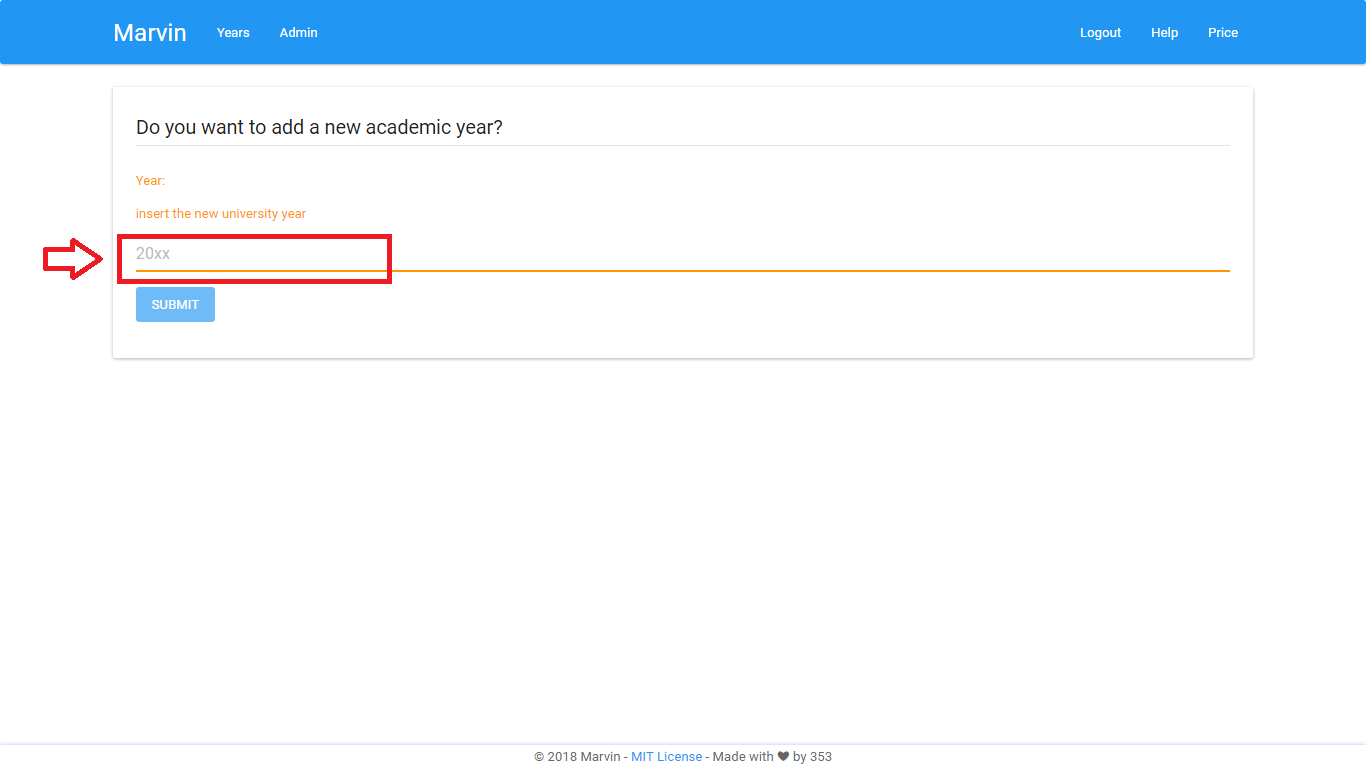
\includegraphics[width=0.7\linewidth]{image/UniversityAddYear1}
		\caption[Add year form]{Fill the form}
		\label{fig:Add a new academic year, fill the form}
	\end{figure}
	\item Click on the button ``Submit".
	\begin{figure}[H]
		\centering
		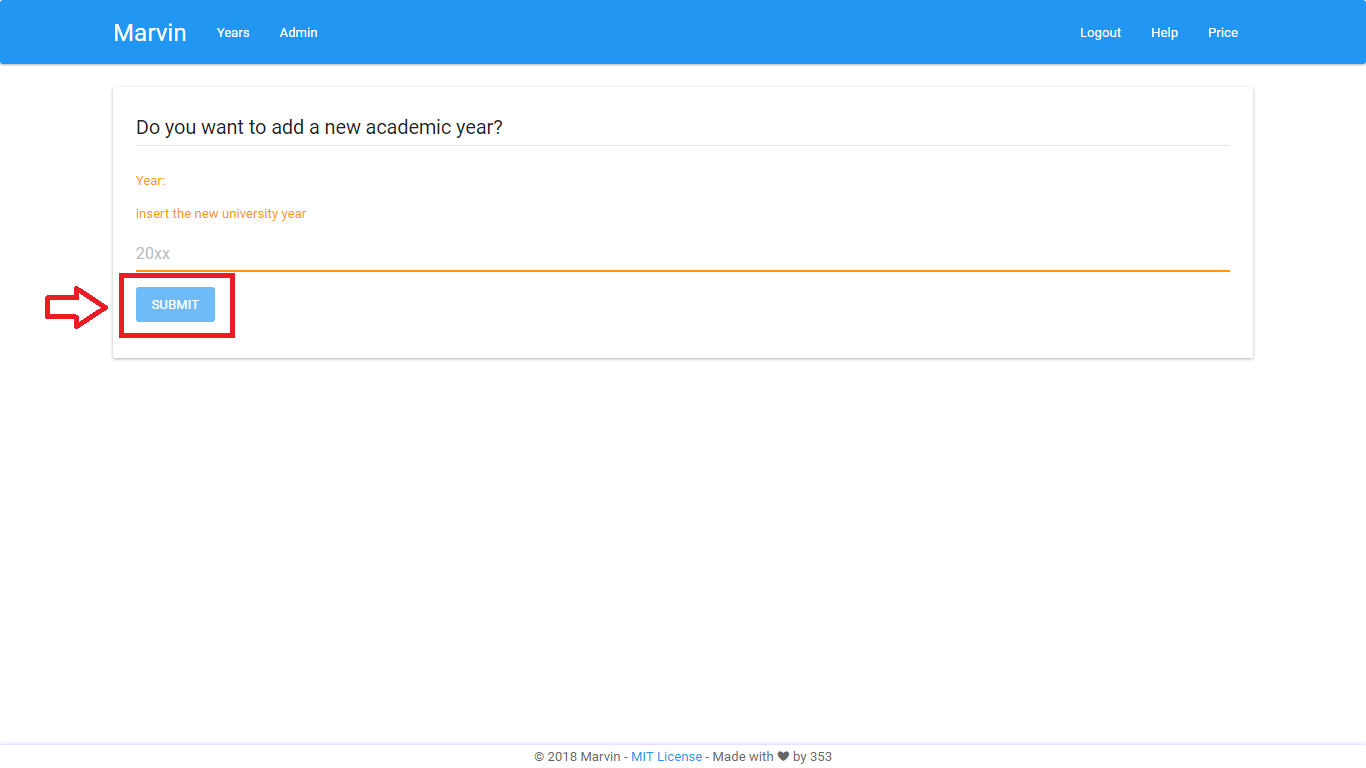
\includegraphics[width=0.7\linewidth]{image/UniversityAddYear2}
		\caption[Add year submit]{Click submit}
		\label{fig:CLick submit}
	\end{figure}
\end{enumerate}

\subsection{Remove an academic year}
Only the years that do not contain courses can be removed, the attempt to remove a year containing at least one course will be reported as incorrect by Metamask.\\
To remove an academic year, you must go to the manage academic years' section and click on the "DELETE" button next to the year you want to delete.
\begin{figure}[H]
	\centering
	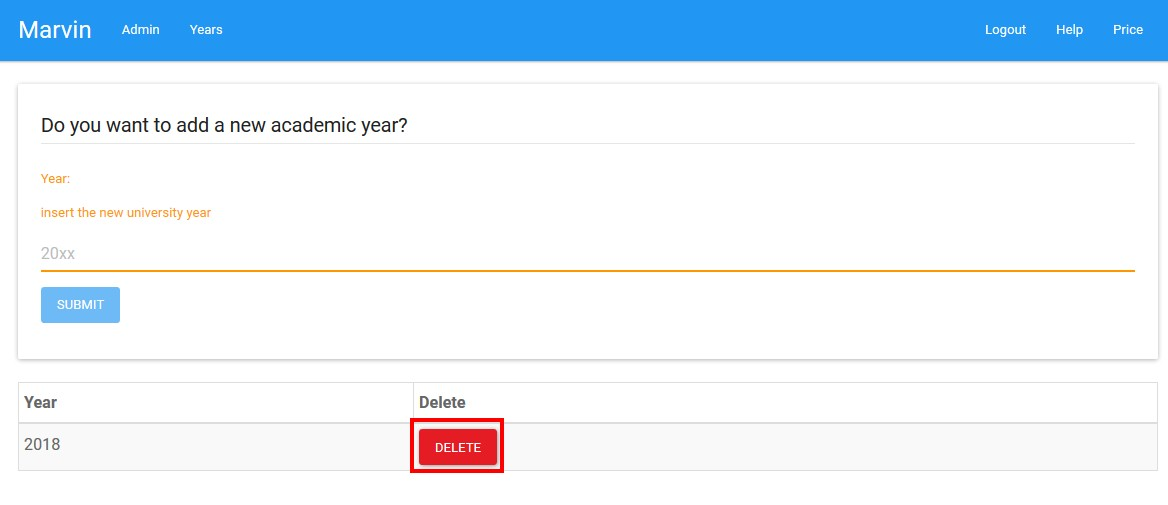
\includegraphics[width=0.7\linewidth]{image/UniversityRemoveYear1}
	\caption[Add year form]{Remove the year}
	\label{fig:Remove the year}
\end{figure}

\end{document}